% Standalone TikZ figure: Parameter Space Taxonomy Visualization
% For Chapter 1: Introduction - Section 1.3 Problem Formulation
\documentclass[tikz,border=10pt]{standalone}
\usepackage{tikz}
\usepackage{amsmath}
\usetikzlibrary{arrows.meta, positioning, shapes.geometric, decorations.pathreplacing, calc}

\begin{document}
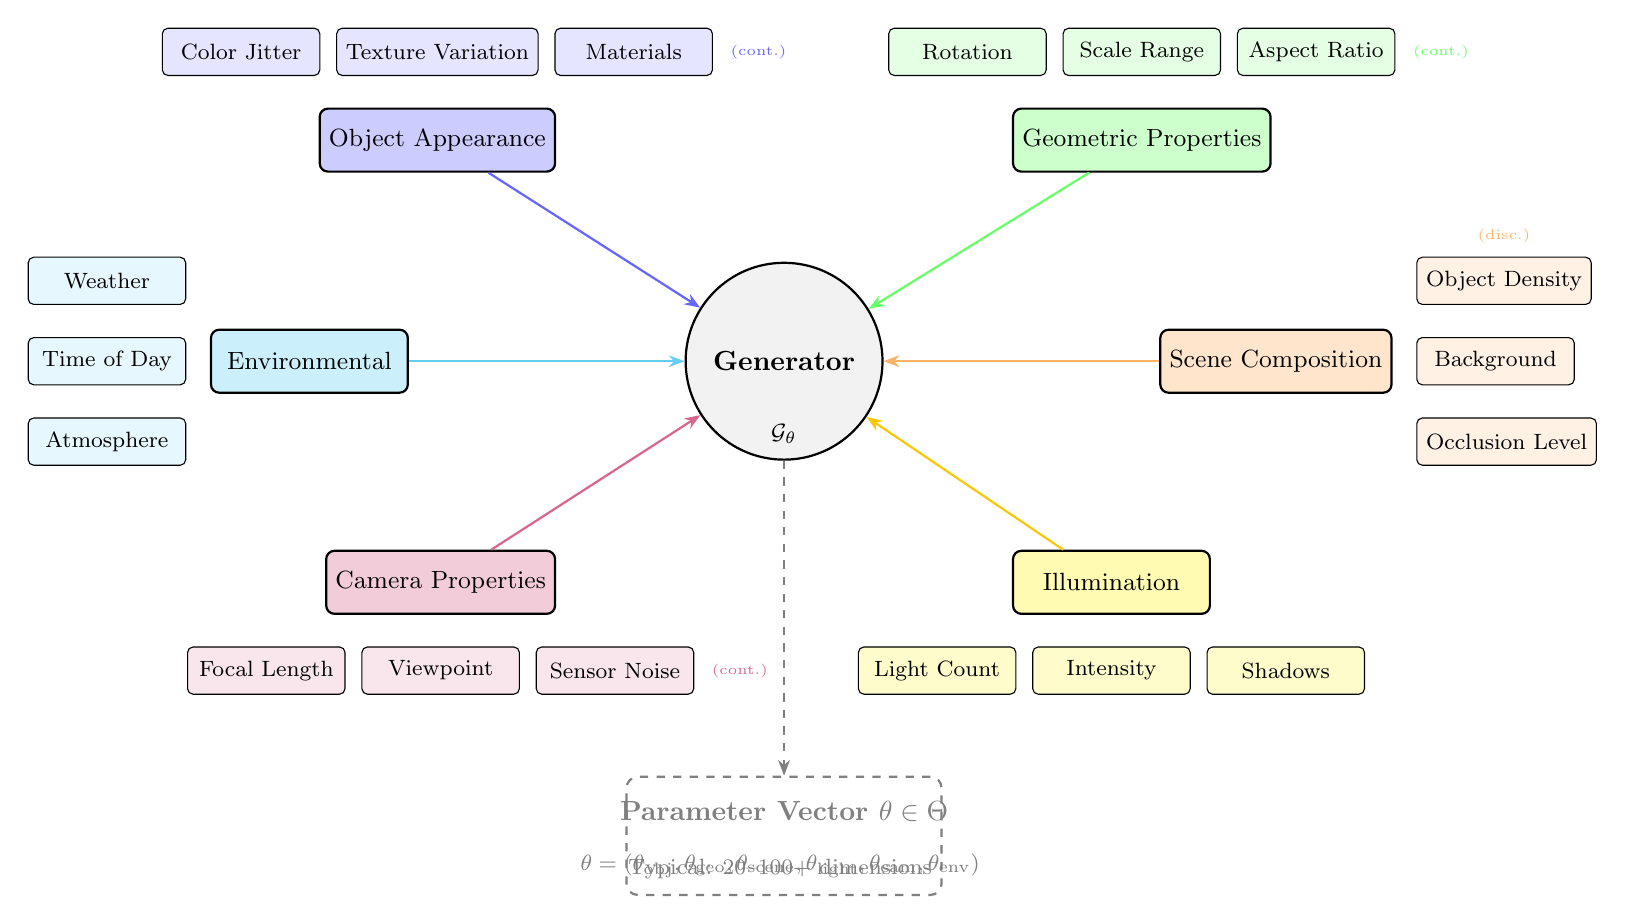
\begin{tikzpicture}[
    node distance=0.8cm,
    every node/.style={font=\small},
    category/.style={rectangle, draw, thick, minimum width=2.5cm, minimum height=0.8cm, align=center, rounded corners=3pt, fill=#1},
    param/.style={rectangle, draw, minimum width=2cm, minimum height=0.6cm, align=center, rounded corners=2pt, font=\footnotesize, fill=#1},
    arrow/.style={-{Stealth[length=2mm]}, thick},
    brace/.style={decorate, decoration={brace, amplitude=5pt, raise=3pt}},
    title/.style={font=\bfseries}
]

% Central node
\node[draw, thick, circle, minimum size=2.5cm, fill=gray!10] (center) {};
\node[title] at (center.center) {Generator};
\node[font=\footnotesize] at (center.south) [above=0.1cm] {$\mathcal{G}_\theta$};

% Object Appearance (top-left)
\node[category=blue!20, above left=1.5cm and 2cm of center] (obj_app) {Object Appearance};
\node[param=blue!10, above=0.4cm of obj_app] (tex) {Texture Variation};
\node[param=blue!10, left=0.2cm of tex] (col) {Color Jitter};
\node[param=blue!10, right=0.2cm of tex] (mat) {Materials};
\draw[arrow, blue!60] (obj_app) -- (center);

% Geometric Properties (top-right)
\node[category=green!20, above right=1.5cm and 2cm of center] (geo) {Geometric Properties};
\node[param=green!10, above=0.4cm of geo] (scale) {Scale Range};
\node[param=green!10, left=0.2cm of scale] (rot) {Rotation};
\node[param=green!10, right=0.2cm of scale] (asp) {Aspect Ratio};
\draw[arrow, green!60] (geo) -- (center);

% Scene Composition (right)
\node[category=orange!20, right=3.5cm of center] (scene) {Scene Composition};
\node[param=orange!10, above right=0.3cm and 0.3cm of scene] (dens) {Object Density};
\node[param=orange!10, below right=0.3cm and 0.3cm of scene] (occ) {Occlusion Level};
\node[param=orange!10, right=0.3cm of scene] (bg) {Background};
\draw[arrow, orange!60] (scene) -- (center);

% Illumination (bottom-right)
\node[category=yellow!30, below right=1.5cm and 2cm of center] (light) {Illumination};
\node[param=yellow!20, below=0.4cm of light] (int) {Intensity};
\node[param=yellow!20, left=0.2cm of int] (lcount) {Light Count};
\node[param=yellow!20, right=0.2cm of int] (shadow) {Shadows};
\draw[arrow, yellow!60!orange] (light) -- (center);

% Camera Properties (bottom-left)
\node[category=purple!20, below left=1.5cm and 2cm of center] (cam) {Camera Properties};
\node[param=purple!10, below=0.4cm of cam] (view) {Viewpoint};
\node[param=purple!10, left=0.2cm of view] (focal) {Focal Length};
\node[param=purple!10, right=0.2cm of view] (noise) {Sensor Noise};
\draw[arrow, purple!60] (cam) -- (center);

% Environmental (left)
\node[category=cyan!20, left=3.5cm of center] (env) {Environmental};
\node[param=cyan!10, above left=0.3cm and 0.3cm of env] (weather) {Weather};
\node[param=cyan!10, below left=0.3cm and 0.3cm of env] (atmos) {Atmosphere};
\node[param=cyan!10, left=0.3cm of env] (tod) {Time of Day};
\draw[arrow, cyan!60] (env) -- (center);

% Parameter space annotation
\node[draw, dashed, rounded corners, thick, gray,
      minimum width=4cm, minimum height=1.5cm,
      below=4cm of center] (theta) {};
\node[title, gray] at (theta.north) [below=0.2cm] {Parameter Vector $\theta \in \Theta$};
\node[font=\footnotesize, gray, align=center] at (theta.center) [below=0.1cm] {
    $\theta = (\theta_{\text{obj}}, \theta_{\text{geo}}, \theta_{\text{scene}}, \theta_{\text{light}}, \theta_{\text{cam}}, \theta_{\text{env}})$
};

% Dimension annotation
\node[font=\footnotesize, gray, align=center] at (theta.south) [above=0.1cm] {
    Typical: 20--100+ dimensions
};

% Connect center to theta
\draw[arrow, gray, dashed] (center.south) -- (theta.north);

% Type annotations
\node[font=\tiny, blue!60, right=0.1cm of mat] {(cont.)};
\node[font=\tiny, green!60, right=0.1cm of asp] {(cont.)};
\node[font=\tiny, orange!60, above=0.05cm of dens] {(disc.)};
\node[font=\tiny, purple!60, right=0.1cm of noise] {(cont.)};

\end{tikzpicture}
\end{document}
